\documentclass[12pt]{exam}

\usepackage{amsmath}
\usepackage[brazil]{babel}
% \usepackage[latin1]{inputenc}
\usepackage[utf8]{inputenc}
\usepackage{graphicx}
\usepackage{url,color}
\usepackage{xcolor}
\usepackage{geometry}
\usepackage{array}
\usepackage{listings}
% \usepackage{minted}
\usepackage{tikz}
% \usepackage{minted}

\def\width{18}
\def\hauteur{13}

\usepackage{enumerate,mdwlist}


\geometry{a4paper, left=2cm, right=2cm, bottom=2.7cm}

\noprintanswers

\renewcommand{\solutiontitle}{\noindent\textbf{Resposta:}\enspace}

\newcolumntype{P}[1]{>{\centering\arraybackslash}p{#1}}
\newcolumntype{M}[1]{>{\centering\arraybackslash}m{#1}}
\newcolumntype{L}[1]{>{\raggedright\arraybackslash}p{#1}}
\newcolumntype{R}[1]{>{\raggedleft\arraybackslash}p{#1}}

\lstset{ 
	language=C, % choose the language of the code
	basicstyle=\fontfamily{pcr}\selectfont\color{black}\small,
	keywordstyle=\color{blue}\bfseries, % style for keywords
	numbers=none, % where to put the line-numbers
	numberstyle=\tiny, % the size of the fonts that are used for the line-numbers     
	showspaces=false, % show spaces adding particular underscores
	showstringspaces=false, % underline spaces within strings
	showtabs=false, % show tabs within strings adding particular underscores
	frame=none, % adds a frame around the code
	tabsize=2, % sets default tabsize to 2 spaces
	rulesepcolor=\color{gray},
	rulecolor=\color{black},
	captionpos=b, % sets the caption-position to bottom
	breaklines=true, % sets automatic line breaking
	breakatwhitespace=false, 
}

\lstset{
	literate=%
	{á}{{\'a}}1
	{â}{{\^a}}1
	{ã}{{\~a}}1
	{í}{{\'i}}1
	{é}{{\'e}}1
	{ý}{{\'y}}1
	{ú}{{\'u}}1
	{ó}{{\'o}}1
	{ě}{{\v{e}}}1
	{š}{{\v{s}}}1
	{č}{{\v{c}}}1
	{ç}{{\c{c}}}1
	{ř}{{\v{r}}}1
	{ž}{{\v{z}}}1
	{ď}{{\v{d}}}1
	{ť}{{\v{t}}}1
	{ň}{{\v{n}}}1                
	{ů}{{\r{u}}}1
	{Á}{{\'A}}1
	{Í}{{\'I}}1
	{É}{{\'E}}1
	{Ý}{{\'Y}}1
	{Ú}{{\'U}}1
	{Ó}{{\'O}}1
	{Ě}{{\v{E}}}1
	{Š}{{\v{S}}}1
	{Č}{{\v{C}}}1
	{Ř}{{\v{R}}}1
	{Ž}{{\v{Z}}}1
	{Ď}{{\v{D}}}1
	{Ť}{{\v{T}}}1
	{Ň}{{\v{N}}}1                
	{Ů}{{\r{U}}}1    
}

\firstpageheader{\includegraphics[width=1.6cm]{logo1.png}}{\textbf{\hspace{1cm} Instituto Federal de Educação, Ciência e Tecnologia de Santa Catarina} \\
\textbf{Departamento Acadêmico de Eletrônica}}
{}

\lfoot{}
\rfoot{}
\cfoot{}

\footer{}{\textbf{Página \thepage\ de 1}}{}

\pointsinmargin


\begin{document}

\vspace{2cm}

\begin{questions}

	\question Diagrama:

	\begin{figure}[!htb]
		\centering
		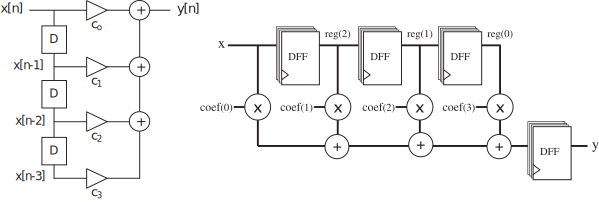
\includegraphics[scale=1]{fir.pdf}
		\caption{Diagrama e RTL do filtro FIR}
		\label{fig:fir}
	\end{figure}

	\question Equação:

	\begin{eqnarray}
		y[n] = \sum_{k=0}^{M}c_kx[n-k]
	\end{eqnarray}

	\question Exemplo de arquivo de entrada:

	\begin{verbatim}
	(hex) 00  34  EF 67  16 38 53  F0 4B  E1   EF  FF  9A  FF  A6  CE (...)
	(dec) 0   52 -17 103 22 56 83 -16 75 -31  -17 -1  -102 -1 -60 -50
	\end{verbatim}


	\question Todos os coeficientes = 1, dividindo por 4 no final.

	\begin{eqnarray}
		y[0] &=& c[0] . x[0] = 52 . 1 = 52/4 = 13 \nonumber \\
		y[1] &=& c[0] . x[1] + c[1] . x[0] = -17 + 52 = 35 / 4 = 8 \nonumber \\
		y[2] &=& c[0] . x[2] + c[1] . x[1] + c2 . x[0] = 103 - 17 + 52 = 138/4 = 34 \nonumber \\
		y[3] &=& c[0] . x[3] + c[1] . x[2] + c2 . x[1] + c3 . x[0] = 22 + 103 - 17 + 52 = 160/4 = 40 \nonumber \\
		y[4] &=& c[0] . x[4] + c[1] . x[3] + c2 . x[3] + c3 . x[1] = 56 + 22 + 103 - 17 = 164/4 = 41 \nonumber \\
		y[5] &=& \dots \nonumber
	\end{eqnarray}

	\question Exemplo de arquivo de saída:

	\begin{verbatim}
	(hex) 00 0D 08 22 28 29 42 24 31 1B 02 06 DA E1 (...)
	(dec) 00 13  8 34 40 41 66 36 49 27 2 6 -38 -31 (...)
	\end{verbatim}


	\question Fonte de audio teste440\_2000 (tom em 440Hz e 2000Hz):

	\begin{figure}[!htb]
		\centering
		\includegraphics[scale=1]{teste440_2000.png}
		\caption{Sinal de entrada: 440 e 2000Hz.}
		\label{fig:fir1}
	\end{figure}

	\begin{figure}[!htb]
		\centering
		\includegraphics[scale=1]{saida_teste440_2000.png}
		\caption{Saída pós filtro.}
		\label{fig:fir1}
	\end{figure}

\end{questions}

\newpage 

Referências:

\vspace{0.5cm}

Pedroni, Volnei A. \textbf{Circuit design with VHDL}. MIT Press, 2004.

Ocenaudio. \url{https://www.ocenaudio.com/}

\end{document}
